% =========================================================
%  Toward Interaction Dynamics: A Predictive Framework for Safe pHRI
%  Author version (de-anonymized) for arXiv
% =========================================================
\documentclass[journal]{IEEEtran}

\usepackage{amsmath,amssymb,amsfonts}
\usepackage{amsthm}
\usepackage{graphicx}
\usepackage{booktabs}
\usepackage{bm}
\usepackage{cite}
\usepackage{enumitem}
\usepackage[colorlinks=true,linkcolor=blue,citecolor=blue,urlcolor=blue]{hyperref}

\interdisplaylinepenalty=2500

\newtheorem{theorem}{Theorem}
\newtheorem{proposition}{Proposition}
\newtheorem{corollary}{Corollary}
\newtheorem{remark}{Remark}
\newtheorem{definition}{Definition}

% Convenience macros
\newcommand{\Lam}{\Lambda(q)}
\newcommand{\Laminv}{\Lambda^{-1}(q)}
\newcommand{\Fmpc}{F_{\text{mpc}}}
\newcommand{\Fmpck}[1]{F_{\text{mpc},#1}}
\newcommand{\dhat}{\hat{d}}
\newcommand{\Jvb}{\bar{J}_v}
\newcommand{\Nbar}{\bar{N}}

% Tighten spacing around floats and captions to save vertical space
\setlength{\textfloatsep}{6pt plus 2pt minus 2pt}
\setlength{\floatsep}{5pt plus 2pt minus 2pt}
\setlength{\intextsep}{5pt plus 2pt minus 2pt}
\setlength{\dbltextfloatsep}{7pt plus 2pt minus 2pt}
\setlength{\abovecaptionskip}{3pt}
\setlength{\belowcaptionskip}{0pt}
\setlength{\abovedisplayskip}{4pt plus 1pt minus 1pt}
\setlength{\belowdisplayskip}{4pt plus 1pt minus 1pt}
\setlength{\abovedisplayshortskip}{2pt plus 1pt}
\setlength{\belowdisplayshortskip}{2pt plus 1pt}

% --- compress reference list to fit the page budget ---
\let\OLDthebibliography\thebibliography
\renewcommand\thebibliography[1]{%
  \footnotesize
  \OLDthebibliography{#1}%
  \setlength{\itemsep}{-1.5pt}%
  \setlength{\parsep}{0pt}%
  \setlength{\topsep}{0pt}%
}

\begin{document}

% ----------------------------------------------------------
\title{Toward Interaction Dynamics: A Predictive Framework for Safe Physical Human–Robot Interaction}

\author{Yongyan~Cao$^{1}$ and Jinshan~Tang$^{2}$%
\thanks{$^{1}$Y. Cao is with Voryx Robotics LLC, San Jose, CA 95136, USA
(e-mail: yongyancao@gmail.com).}%
\thanks{$^{2}$J. Tang is with the Department of Health Administration and
Policy, George Mason University, Fairfax, VA, USA
(e-mail: jtang25@gmu.edu).}}

\maketitle

% ----------------------------------------------------------
\begin{abstract}
Safe physical human--robot interaction (pHRI) requires tracking a
commanded motion, yielding under human forces, respecting actuator and
joint limits, and staying predictable under persistent contact.
Classical impedance control trades accuracy for safety: a sustained
force produces the steady-state bias $e_\infty=-K_d^{-1}F_h$.
We propose a predictive framework that models the interaction error
itself: an operational-space feedforward cancels gravity and Coriolis
terms and normalizes the task inertia, leaving a linear
interaction-dynamics backbone --- a double-integrator reduction of the
interaction error --- whose state-transition matrix is
configuration-independent.
This converts nonlinear torque-controlled pHRI into a linear
constrained-control problem: offset-free tracking, actuator feasibility,
quadratic stabilizability over a certified polytope of configurations,
and sampled-data joint-limit safety follow from a 30-variable convex QP
at 100\,Hz with a Kalman filter that rejects persistent forces without
steady-state error.
In MuJoCo simulation of a 7-DOF Franka FR3, it reduces steady-state
error under a sustained 15\,N force from 44.8\,mm to below 0.05\,mm,
holds sub-millimeter tracking on four 3-D circles, and is robust to
position-measurement noise and up to 30\% inertial mismatch.
Because the backbone reduces contact to a linear model with a fixed
transition matrix, it may serve as a dynamics prior for model-based
physical AI.
\end{abstract}

\begin{IEEEkeywords}
Interaction dynamics, impedance control, model predictive control,
physical human--robot interaction, disturbance rejection, joint-limit
safety, redundant manipulator.
\end{IEEEkeywords}

% ----------------------------------------------------------
\section{Introduction}

Robots are moving from structured, isolated workcells into continuous
physical contact with people and unstructured environments---collaborative
assembly, assistive and rehabilitation devices, surgical robots, and service
robots all require the machine to stay safe and predictable while executing a
precise task~\cite{villani2016force,albu2007unified,haddadin2009requirements}.
In these settings the quality of the physical interaction is not a secondary
concern but a primary control objective.

Classical robot control is organized around \emph{robot} dynamics: trajectory
tracking, inverse dynamics, and whole-body control take the manipulator as the
principal dynamical system and treat contact forces as external disturbances
or constraints~\cite{khatib1987unified}. This is highly effective in free
space but becomes restrictive once interaction dominates behavior, because the
object the controller reasons about---the robot's configuration-space
dynamics---is not the object the task cares about, namely the \emph{interaction}
at the contact port. This motivates a shift in modeling emphasis: rather than
predict robot motion and react to interaction, we make the \emph{interaction
dynamics}---the closed-loop relation among commanded motion, contact
force, actuator and joint limits, and safety filters at the contact port---the quantity that is
explicitly modeled, predicted, and optimized (formalized in Definition~\ref{def:id}). We use
the term in a deliberately specific modeling sense---the augmented
error-and-force state at the contact port taken as the object of prediction
and constraint---not as a claim to a new physical phenomenon; it is closely
related to the operational-space and error-dynamics
formulations~\cite{khatib1987unified,siciliano2009robotics} and differs from
them in \emph{what is treated as the modeled state} (the interaction error, not
the configuration) rather than in the underlying mechanics. This paper develops
one concrete, offset-free predictive realization of it.

Impedance and admittance control are the dominant pHRI
paradigms~\cite{hogan1985impedance,chiaverini1999survey}: they prescribe a
desired dynamic relation between motion and contact force and are valued for
their simplicity and physical
transparency~\cite{villani2016force,albu2007unified}. Two limitations persist.
First, they are fundamentally \emph{reactive}---the desired port behavior is
enforced by feedback after the force acts, and a fixed stiffness fixes the
accuracy--safety trade-off: under a sustained force the steady-state deflection
is $e_\infty=-K_d^{-1}F_h$ (a 15\,N push through 300\,N/m gives 50\,mm), so
stiffening for accuracy raises contact force~\cite{haddadin2009requirements}
while integral action removes the bias only within a narrow stable-gain budget
and is prone to windup~\cite{cao2004antiwindup,cao2002antiwindup}. Second, task
tracking, interaction shaping, and constraints are typically designed in
separate modules, precluding a single optimization.

Model predictive control (MPC) addresses the second gap by folding
constraints, actuator limits, and future prediction into one
optimization~\cite{mayne2000constrained,mayne2014model}, and offset-free MPC
removes steady-state error by augmenting an integrating disturbance state
estimated by a Kalman filter~\cite{pannocchia2003disturbance}. Yet most
impedance-MPC formulations either optimize impedance \emph{parameters}---which
enter the prediction nonlinearly and cap update rates at
10--30\,Hz~\cite{cao2023passive,haninger2023model,roveda2019optimal}---or
compensate the estimated disturbance only reactively at the current
step~\cite{wu2025ensuring}. Variable impedance
methods~\cite{liu2025model,ikeura1995variable} adapt the apparent stiffness but
likewise give no offset-free guarantee under persistent unknown force. What is
missing is a formulation in which the interaction error itself is the linear
dynamical object exposed to standard constrained-control machinery.

Our hypothesis is that safe interaction is best posed on a predictive
representation of the interaction error, in which impedance behavior is not a
separate controller but an emergent property of the optimized dynamics.
Computed-torque and operational-space linearization to a double integrator are
classical~\cite{khatib1987unified,siciliano2009robotics}; the contribution here
is to make that reduction the \emph{backbone} of the predictive interaction
problem. An operational-space feedforward cancels gravity and Coriolis terms
and normalizes the task through the operational-space inertia, leaving a
residual task-error double integrator whose discrete state-transition matrix
$A_d$ is \emph{constant}, with all robot configuration dependence isolated in
the input matrix $B_d(\rho_k)$---the scheduling-dependent structure familiar
from LPV predictive control~\cite{cao2005minmax}.

This paper makes four contributions:

\textbf{A predictive interaction-dynamics formulation.} We recast
torque-controlled pHRI so that the modeled and optimized object is the
interaction error at the contact port rather
than the robot configuration dynamics, unifying compliance, tracking,
disturbance rejection, and safety in one convex program while preserving the
measured robot dynamics through $M$, $C\dot q+G$, and $J_v$.

\textbf{A configuration-independent state-transition matrix.} Operational-space
feedforward cancellation makes the discrete transition matrix $A_d$ \emph{constant}
across all configurations, confining the entire robot dependence to the input
(control-effectiveness) matrix $B_d(\rho_k)$---the classical LPV structure in
which $A$ is fixed and only $B$ is scheduled. This lets the free-response matrix
be precomputed once, keeps the online problem a fixed 30-variable QP at 100\,Hz
at every configuration, and reduces the LPV backbone's closed-loop stability to
a finite vertex LMI certifying quadratic stabilizability, by one fixed
feedback gain, over a polytope of configurations
(Theorem~\ref{thm:workspace}) rather than only at a frozen configuration ---
a statement about the backbone under that certified gain, not directly about
the deployed receding-horizon MPC.

\textbf{Offset-free predictive impedance.} We prove
(Theorem~\ref{thm:equiv}) that classical task-space
impedance~\cite{hogan1985impedance} is a \emph{special case} of this
framework---in the unconstrained, disturbance-free limit the predictive
feedback reduces to it for the passive symmetric component of the realized
gain---and (Theorem~\ref{thm:zss}) that an input-centered augmented-Kalman
disturbance state gives zero steady-state error under constant bounded human
force when the stated stability and feasibility conditions hold, removing the
fixed accuracy--safety trade-off of impedance control.

\textbf{Safety and passivity integration.} A null-space
inverse-barrier potential~\cite{sadeghian2014task}, a one-step joint-limit
control-barrier filter on the final applied torque, and an energy-tank scaling
of the predictive task force provide practical joint-limit regulation and
sampled task-channel passivity, \emph{conditional} on feasibility and
per-sample enforcement.

On a 7-DOF Franka FR3 in MuJoCo simulation, the controller reduces
steady-state error under a sustained 15\,N force from 44.8\,mm (classical
impedance) to below 0.05\,mm---a $>$800$\times$ reduction---while holding
sub-millimeter tracking on four 3-D circles and remaining robust to
position-measurement noise and up to 30\% inertial mismatch. Although developed for pHRI, the
interaction-dynamics backbone requires only $M$, $C\dot q+G$, and $J_v$,
offering a path toward interaction models that transfer across configurations
for manipulation and whole-body control; a full realization of that vision is
left to future work.

The same analytic reduction points toward an interaction-dynamics prior for
\emph{model-based physical AI}; we return to this in the conclusion rather than
claim it here.

% ----------------------------------------------------------
\section{System Dynamics and Problem Formulation}

Consider an $n$-DOF torque-controlled serial manipulator; experiments
use the Franka FR3 ($n=7$)~\cite{franka2023fr3}.
The rigid-body equations of motion are:
\begin{equation}\label{eq:eom}
  M(q)\ddot{q}+C(q,\dot{q})\dot{q}+G(q)=\tau+J^\top(q)\mathcal{F}_h
\end{equation}
where $M(q)$ is the positive-definite inertia matrix;
$C(q,\dot{q})\dot{q}+G(q)$ is the Coriolis-plus-gravity vector
(available as \texttt{qfrc\_bias} in MuJoCo or via the robot model API);
$\tau$ is the commanded joint torque; and $\mathcal{F}_h\in\mathbb{R}^6$
is the human-applied wrench.
$J(q)=[J_v^\top(q);\;J_\omega^\top(q)]^\top\in\mathbb{R}^{6\times n}$
is the full geometric Jacobian, with $J_v\in\mathbb{R}^{3\times n}$ the
translational and $J_\omega\in\mathbb{R}^{3\times n}$ the rotational
sub-Jacobian~\cite{siciliano2009robotics}.
$\mathcal{F}_h$ is defined as positive when the human pushes
\emph{onto} the robot, so it enters~\eqref{eq:eom} with a positive
sign, adding to the generalized force that accelerates the joints.

The translational Jacobian satisfies $\dot{p}=J_v(q)\dot{q}$~%
\cite{siciliano2009robotics}.
The operational-space inertia~\cite{khatib1987unified} is:
\begin{equation}\label{eq:Lambda}
  \Lambda(q)=\bigl(J_vM^{-1}J_v^\top\bigr)^{-1}\in\mathbb{R}^{3\times3}
\end{equation}
$\Lambda(q)$ is symmetric positive-definite.
The dynamically-consistent
pseudoinverse~\cite{khatib1987unified,sentis2005synthesis} is
$\Jvb=M^{-1}J_v^\top\Lambda$, ensuring forces applied through
$J_v^\top$ produce no null-space acceleration.

After feedforward cancellation (Section~\ref{sec:layer1}), the human
force and joint friction appear as an aggregated Cartesian
\emph{acceleration} disturbance $d_{\text{acc}}(t)$ (units m/s$^2$ ---
kept notationally distinct throughout from its \emph{force}-equivalent
$d$, units N, introduced in Section~\ref{sec:layer2c} and used from Layer
2 onward), modelled as a random walk:
\begin{equation}\label{eq:distmodel}
  \dot{d}_{\text{acc}}=w(t),\quad w\sim\mathcal{N}(0,Q_d)
\end{equation}
capturing constant forces (sustained pushes, physiological tremor) and
slow-varying loads (unmodelled payloads, tool changes).
This decomposition is written in acceleration units; the estimator and QP of
Section~\ref{sec:layer2} operate on the equivalent \emph{force-form}
disturbance $-\Lambda(q)\,d$ (the quantity entering through $B_d(\rho_k)$ in
\eqref{eq:augstate}), which is constant for a constant human force and is the
form realized in code.

Our control objective can be stated as follows. 
Design a torque law $\tau$ such that for any bounded persistent
disturbance $d$:
\begin{enumerate}
  \item $\|e(\infty)\|=0$, where $e=p_d-p$ (zero steady-state error);
  \item $\|e(t)\|$ is minimized over a finite prediction horizon;
  \item $q_i\in[q_{\min,i}+\epsilon,\;q_{\max,i}-\epsilon]$
        for all $i$ when the one-step safety filter is enforced.
\end{enumerate}

This objective is posed not on the robot configuration but on the interaction
error at the contact port. We make that modeling shift precise.

\begin{definition}[Interaction Dynamics]\label{def:id}
We call \emph{interaction dynamics} the closed-loop dynamical system whose
state is the interaction error at the contact port---the task-tracking error
and its rate, augmented by the persistent interaction force---and whose
evolution, under the actuator, joint-limit, and passivity constraints, is
driven by the task control input. Formally, where classical robot control takes
the configuration-space dynamics \eqref{eq:eom} as the object to be predicted and regulated,
interaction dynamics takes the augmented error system
\[
  x_{k+1} = A\,x_k + B\,u_k + E\,d_k
\]
as the primary modeling object, with $x_k$ the interaction error state, $u_k$
the task force, and $d_k$ the interaction disturbance.
\end{definition}

What distinguishes this from a bare tracking-error double integrator is not the
state equation in isolation but the \emph{object} it defines: the error, the
interaction force (as an estimated, internally-modeled disturbance state rather
than an exogenous input), and the actuator, joint-limit, and passivity
constraints are taken together as one predicted-and-optimized system. Plain
error dynamics describe how a fixed controller's error evolves; the interaction
dynamics of Definition~\ref{def:id} are the object the controller is designed
\emph{on}.

Section~\ref{sec:layer2} constructs one concrete, offset-free realization of
this object: the transition matrix $A=A_d$ is configuration-independent, the
robot dependence is confined to $B=B_d(\rho_k)$, and $E$ propagates the
estimated interaction force. Modeling the \emph{interaction} rather than the
\emph{configuration} is what lets compliance, tracking, disturbance rejection,
and safety be posed as a single constrained optimization.

% ----------------------------------------------------------
\section{Linear Interaction-Dynamics Backbone and Finite-Horizon Realization}

\subsection{Layer 1 --- Feedforward Nonlinear Inversion}
\label{sec:layer1}

Classical Cartesian impedance control~\cite{hogan1985impedance} commands:
\begin{equation*}
  \tau = C\dot{q}+G+J_v^\top(\Lambda\ddot{p}_d+\mu-K_de-D_d\dot{e})
\end{equation*}
where $\mu=\Lambda J_vM^{-1}C\dot{q}-\Lambda\dot{J}_v\dot{q}$ collects
task-space Coriolis and centripetal terms~\cite{khatib1987unified},
embedding the full impedance law inside a single static feedback.
This treats $F_h$ as a disturbance to be passively rejected with no
predictive look-ahead and no mechanism to drive steady-state error to
zero.

The proposed Layer~1 explicitly separates these concerns.
Following the operational-space decomposition of~\cite{khatib1987unified},
the full torque command is partitioned into four channels via the
null-space projector $\Nbar=I-\bar{J}J$~\cite{sentis2005synthesis}, where
$\bar{J}=M^{-1}J^\top\Lambda_6$ is the dynamically-consistent pseudoinverse
of the full $6$-DOF pose Jacobian $J$ and
$\Lambda_6=(JM^{-1}J^\top)^{-1}\in\mathbb{R}^{6\times6}$ is the full-pose
operational-space inertia (both the translational MPC task and the
orientation channel are actively controlled, so the projector annihilates
the full pose task, not only its translational part):
\begin{equation}\label{eq:tau}
  \tau = \tau_{\text{ff}}+J_v^\top\Fmpc
        +J_\omega^\top F_{\text{orient}}+\Nbar^\top\tau_{\text{null}}
\end{equation}

The feedforward term cancels all known nonlinearities using the
computed-torque method~\cite{siciliano2009robotics}:
\begin{equation}\label{eq:tff}
  \tau_{\text{ff}} = \underbrace{C(q,\dot{q})\dot{q}+G(q)}_{\texttt{qfrc\_bias}}
                   + J_v^\top\Lambda(q)\,\ddot{p}_d
\end{equation}

Writing the Layer-2 task channel as $\tau_{\text{mpc}}\equiv J_v^\top\Fmpc$,
define the known non-MPC torque offset
\[
  \tau_{\text{base}}=
  \tau_{\text{ff}}+J_\omega^\top F_{\text{orient}}+\Nbar^\top\tau_{\text{null}}.
\]
The final applied command is the joint torque
$\tau = \tau_{\text{base}}+\tau_{\text{mpc}}$, which the hardware saturates at
the per-joint actuator limit $|\tau_i|\leq\tau_{\max,i}$; Layer~2 constrains
this applied receding-horizon torque, while the hardware interface keeps
clipping and rate limiting as final runtime guards.

\begin{proposition}\label{prop:doubleint}
After applying \eqref{eq:tff}, the residual error dynamics are represented by
the linear double integrator
\begin{equation}\label{eq:errordyn}
  \ddot{e} = -\Laminv\,\Fmpc + d_{\text{acc}}(t)
\end{equation}
with $e=p_d-p$; every term left over from the feedforward cancellation ---
not just the human force --- is collected into the \emph{acceleration}-form
disturbance $d_{\text{acc}}(t)$, defined below (not to be confused with its
force-equivalent $d=-\Lambda(q)d_{\text{acc}}$, Section~\ref{sec:layer2c},
which is the quantity actually estimated and cancelled from Layer 2
onward):
\begin{align}\label{eq:dist}
  d_{\text{acc}}(t) &= \underbrace{-\Laminv\,\bar{J}_v^\top J^\top\mathcal{F}_h}_{%
           \text{projected pHRI force}}
          \;\underbrace{-\,J_vM^{-1}J_\omega^\top F_{\text{orient}}}_{%
           \text{orientation coupling}}\notag\\
        &\quad\underbrace{-\,\dot{J}_v(q,\dot{q})\dot{q}}_{%
           \text{Jacobian derivative}}
          \;+\;\underbrace{\epsilon_m(t)}_{\text{model error}}
\end{align}
where $\bar{J}_v^\top=\Lambda J_vM^{-1}\in\mathbb{R}^{3\times n}$ and
$J^\top\in\mathbb{R}^{n\times 6}$ is the full geometric Jacobian transpose,
so $\bar{J}_v^\top J^\top\in\mathbb{R}^{3\times 6}$ acts on the $6$-D wrench
$\mathcal{F}_h$ (equivalently the term is $-J_vM^{-1}J^\top\mathcal{F}_h$).
\end{proposition}

The four terms: (i)~the \emph{projected pHRI force} — for a purely
translational $\mathcal{F}_h=[F_h^\top,0]^\top$ this reduces to
$-\Lambda^{-1}F_h$ in acceleration form (because $e=p_d-p$, any positive
acceleration of $p$ induced by the human force appears with a negative sign
in $\ddot e$);
(ii)~the \emph{orientation coupling} — residual translational
acceleration from the simple additive orientation PD. This mobility
cross-term is generally structural, not a numerical artifact, and is,
in its force-equivalent form, absorbed by $\dhat$;
(iii)~the \emph{Jacobian derivative} $-\dot{J}_v\dot{q}$, small at
typical speeds; (iv)~the \emph{model error} $\epsilon_m(t)$ from
imperfect gravity/Coriolis cancellation.

\begin{remark}[Exactness of the reduction]
Under \emph{ideal} cancellation the residual plant is exactly the double
integrator~\eqref{eq:errordyn}; in practice the terms
(ii)--(iv) are not identically zero. Rather than being neglected they are
\emph{modelled} as the acceleration disturbance $d_{\text{acc}}(t)$, whose
force-equivalent $d=-\Lambda(q)d_{\text{acc}}$ the augmented Kalman state
$\dhat$ estimates and the MPC rejects (Theorem~\ref{thm:zss}). The reduction is
thus a \emph{cancellation-plus-disturbance} model, not an assumption of perfect
inversion; the configuration dependence stays confined to $B_d(\rho_k)$ while
$A_d$ remains constant.
\end{remark}

\subsection{Layer 2 --- Discrete LPV Model and QP}\label{sec:layer2}

With error state $x_e=[e^\top,\dot{e}^\top]^\top\in\mathbb{R}^6$ and
scheduling variable $\rho_k=q_k$, exact zero-order-hold (ZOH) discretization gives:
\begin{equation}\label{eq:lpv}
  x_{e,k+1} = \underbrace{\begin{bmatrix}I_3&\Delta t I_3\\0&I_3\end{bmatrix}}_{A_d\;\text{(constant)}}
              x_{e,k}
            + \underbrace{\begin{bmatrix}-\tfrac{\Delta t^2}{2}\Laminv\\-\Laminv\Delta t\end{bmatrix}}_{B_d(\rho_k)}
              \Fmpck{k}
\end{equation}

Equation~\eqref{eq:lpv}, together with the disturbance augmentation
\eqref{eq:augstate} below, \emph{is} the interaction dynamics of
Definition~\ref{def:id} in concrete form: the state $x_e$ is the interaction
error at the contact port---not the robot configuration---the input $\Fmpc$ is
the task force, and $\hat d$ is the estimated interaction disturbance.
Identifying $A=A_d$ and $B=B_d(\rho_k)$ gives the linear system 
of Definition~\ref{def:id}; offset-free tracking,
actuator feasibility, and joint-limit safety are properties of this model, not
of the configuration dynamics.

\textbf{Structural result.}
The continuous-time matrix $A_c=\begin{bmatrix}0&I_3\\0&0\end{bmatrix}$
is nilpotent ($A_c^2=0$), so the matrix exponential terminates exactly at
first order and $A_d=e^{A_c\Delta t}=I+A_c\Delta t$ is
configuration-independent and exact, with no discretization
approximation; the exact ZOH input integral $B_d(\rho_k)$ is likewise
closed-form. The LPV pair $(A_d,B_d(\rho))$ is uniformly controllable,
and the disturbance state augmented in Sec.~\ref{sec:layer2c} is
detectable, at every configuration away from kinematic singularities
(proof: supplementary material, Sec.~S1, Remark~S1).

\textit{Implementation note (regularization).}
In code $\Lambda^{-1}(q)=J_vM^{-1}J_v^\top+\sigma I$ with $\sigma=10^{-6}$; this
Tikhonov term is negligible in the workspace interior and only mildly damps the
estimate near singularities, outside the operating region.

The receding-horizon QP with $N=10$ steps, $3N=30$ decision variables
$U=[\Fmpck{0};\ldots;\Fmpck{N-1}]$, is:
\begin{subequations}\label{eq:QP}
\begin{align}
  \min_U\;& \tfrac{1}{2}U^\top HU+h^\top U \label{eq:QP_cost}\\
  \text{s.t.}\;&
  -\tau_{\max}\leq
  \tau_{\text{base}}(0)+J_v^\top(q_0)\Fmpck{0}
  \leq\tau_{\max}, \label{eq:QP_torque}\\
  & -F_{\max}\leq\Fmpck{k}\leq F_{\max},
  \quad k=0,\ldots,N-1. \label{eq:QP_force}
\end{align}
\end{subequations}
where $F_{\max}$ is the task-space (Cartesian) corrective-force bound on the
QP's decision variable (distinct from the joint-torque limit $\tau_{\max}$),
and $\tau_{\text{base}}(0)=\tau_{\text{ff}}+J_\omega^\top F_{\text{orient}}+\bar{N}^\top\tau_{\text{null}}$
is the known non-MPC torque offset at the current configuration
(Sec.~\ref{sec:layer1}). $H=\Gamma^\top\bar{Q}\Gamma+\bar{R}$, stage cost
$Q=\text{blkdiag}(K_d,D_d)$, terminal cost $Q_f=\gamma Q$ ($\gamma=5$),
$\bar{Q}=\text{blkdiag}(Q,\ldots,Q,Q_f)$,
$\bar{R}=\text{blkdiag}(R,\ldots,R)$.
Let $d_N=\mathbf 1_N\otimes\dhat$; the linear term is
$h=\Gamma^\top\bar{Q}x_{\text{free}}+\bar R d_N$, corresponding to the
offset-free input-centred effort penalty $\|U+d_N\|_{\bar R}^2$.
The free response $x_{\text{free}}=\Phi x_e+D_{\text{bar}}\dhat$,
where $D_{\text{bar}}\in\mathbb{R}^{6N\times3}$ has $j$-th block
$\sum_{l=0}^{j-1}A_d^l B_d(\rho_k)$; equivalently,
$D_{\text{bar}}=\Gamma(\mathbf 1_N\otimes I_3)$.
Only $\Fmpck{0}$ is applied (receding-horizon principle).
\emph{Constraint interpretation (feasible final control).} The final
applied command is the joint torque
$\tau=\tau_{\text{base}}+J_v^\top\Fmpck{0}$, where
$\tau_{\text{base}}$ contains feedforward, orientation, and null-space terms,
which the hardware saturates at the per-joint actuator limit $\tau_{\max}$
(on the FR3, $\tau_{\max}=[87,87,87,87,12,12,12]$\,Nm). Constraining only the
correction, $\|\Fmpc\|_\infty\leq F_{\max}$, would \emph{not} keep $\tau$
within $\tau_{\max}$: it ignores the feedforward offset $\tau_{\text{ff}}$
(both $C\dot{q}+G$ and the inertial term $J_v^\top\Lambda\ddot{p}_d$, which on
the FR3 dominate the budget), and it bounds a Cartesian force whereas the map
$J_v^\top(q)$ to joint torque is configuration-dependent; any deficit would
be absorbed by a downstream torque clip, i.e.\ \emph{saturation}, discarding
the optimized command. We therefore constrain the first applied
receding-horizon torque directly, as in~\eqref{eq:QP_torque}. Since
$\tau_{\text{base}}(0)$ and $J_v(q_0)$ are known at solve time, the constraint
is affine in $\Fmpck{0}$ --- a convex per-joint polytope solved by OSQP at the
same cost class as a box. As only the first move is applied, the nominal
applied torque satisfies $|\tau_i|\leq\tau_{\max,i}$ whenever the QP is
feasible. Runtime clipping and rate limiting remain as final safety guards;
horizon-wide torque rows can be added but are not required for feasibility of
the applied receding-horizon action. If an over-aggressive reference makes
$\tau_{\text{base}}(0)$ alone exceed $\tau_{\max}$, the constraint could
similarly be softened with a penalized slack $s\geq0$ so the QP stays
feasible and returns a minimum-violation command --- analogous to the
joint-limit CBF relaxation of Sec.~\ref{sec:cbf}, though the present
implementation instead returns a zero correction on infeasibility (see the
correction-authority ablation in the supplementary material, Sec.~S8),
which is simpler but not minimum-violation.

The following result establishes that classical impedance control is not a
competitor to the proposed framework but a special case of it: it is what the
interaction dynamics reduce to once prediction, constraints, and disturbance
augmentation are switched off.

\begin{theorem}[Impedance Equivalence]\label{thm:equiv}
Fix a configuration and assume the input constraints are inactive and
the disturbance estimate is zero. Then the first MPC move is a linear
state feedback
$\Fmpc=K_e e+K_{\dot e}\dot e$. If the realized gain blocks are symmetric
positive definite, or more generally have symmetric parts that define passive
stiffness and damping, set
$K_{\text{eff}}=\operatorname{sym}(K_e)\succ0$ and
$D_{\text{eff}}=\operatorname{sym}(K_{\dot e})\succ0$; the conservative part
of the closed loop is the classical task-space impedance:
\begin{equation}\label{eq:impedance}
  \Lambda(q)\ddot{e}+D_{\text{eff}}\dot{e}+K_{\text{eff}}e = -F_h,
\end{equation}
where $F_h$ is the constant force-equivalent disturbance applied to the
end effector.
\end{theorem}
\begin{proof}
With inactive constraints and $\dhat=0$, \eqref{eq:QP} reduces to an
unconstrained strictly convex quadratic because
$H=\Gamma^\top\bar Q\Gamma+\bar R\succ0$ when $\bar R\succ0$. Its
unique minimizer is
\begin{equation*}
  U^\star=-H^{-1}\Gamma^\top\bar Q\Phi x_e .
\end{equation*}
Let $S=[I_3\;0\;\cdots\;0]$ select the first force block. The applied
force is therefore
\begin{equation*}
  \Fmpc=S U^\star =
  \begin{bmatrix}K_e&K_{\dot e}\end{bmatrix}
  \begin{bmatrix}e\\\dot e\end{bmatrix},
\end{equation*}
for fixed matrices $K_e,K_{\dot e}$ determined by
$(A_d,B_d,\bar Q,\bar R,Q_f,N)$. Under the stated symmetry/sign condition,
the symmetric parts define $K_{\text{eff}}$ and $D_{\text{eff}}$. The exact
linear closed loop is obtained with the full gains $K_e,K_{\dot e}$; only
their symmetric parts admit the conservative spring--damper interpretation.
The skew part of $K_{\dot e}$ is workless gyroscopic damping coupling, whereas
the skew part of $K_e$ is a circulatory position force and is not passive in
general. These skew terms vanish in the common isotropic/commuting case and
are otherwise treated as part of the stabilizing LQR feedback rather than as
classical impedance parameters. The residual plant
from Proposition~\ref{prop:doubleint} is
$\ddot e=-\Lambda^{-1}\Fmpc+d_{\text{acc}}$. For a translational
constant human force represented in force form by $F_h=-\Lambda
d_{\text{acc}}$, multiplication by $\Lambda$ gives
$\Lambda\ddot e=-\Fmpc-F_h$. Substituting the linear feedback yields
\eqref{eq:impedance}.
\end{proof}
Thus the unconstrained MPC realizes a configuration-dependent linear
impedance whenever the gain blocks have the passive stiffness/damping
sign structure; constraints and disturbance augmentation are the
mechanisms that extend this linear impedance behavior.

\begin{remark}[Optimality vs.\ passivity: motivation for the energy tank]
Because the predictive gain is the LQR/Riccati image of $(Q,R)$ rather than a
passive design, the skew part of $K_e$ (Theorem~\ref{thm:equiv}) is a
non-passive circulatory force. For the robot alone this is benign (the DARE
closed loop is asymptotically stable), but coupled to a human---itself a
dynamical system---a non-passive controller need not preserve stability of the
\emph{coupled} loop. This motivates the energy-tank layer of
\S\ref{sec:passivity}: rather than restricting $(Q,R)$ to passive gains and
sacrificing performance, we keep the optimal law and restore a sampled
energy-budget certificate on the scaled translational predictive-force
channel at runtime (Proposition~\ref{prop:tank}), bounding the positive work
that channel can deliver. This is a channel-level certificate, not a
full-port passivity proof (see the scope remark in
\S\ref{sec:passivity}), so it does not by itself guarantee coupled
stability against an arbitrary passive environment; it removes one
identified non-passive source while leaving feedforward, orientation, and
null-space contributions to the port outside its accounting.
\end{remark}

\begin{remark}[Prescribed vs.\ realized gains]\label{rem:gains}
The cost weights $Q=\mathrm{blkdiag}(K_d,D_d)$, $R$ are design
\emph{penalties}; the realized impedance
$(K_{\text{eff}},D_{\text{eff}})$ is their LQR image ---
a nonlinear (Riccati) map of $(Q,R)$ --- so in general
$(K_{\text{eff}},D_{\text{eff}})\neq(K_d,D_d)$. The weights \emph{shape}
the realized impedance: the high-bandwidth tracking reported below
corresponds to the stiff, well-damped $K_{\text{eff}}$ the chosen
$(Q,R)$ induce. If a specific $(K_d,D_d)$ must instead be matched
exactly, the impedance gain can be prescribed directly
($\Fmpc=K_de+D_d\dot{e}$), rendering the equivalence exact for those
gains at the cost of predictive look-ahead. We adopt the LQR form, for
which Theorem~\ref{thm:equiv} already establishes the analytical
connection between the unconstrained MPC and a realized classical
impedance.
\end{remark}

\begin{corollary}[Existence of a Gain-Scheduled Infinite-Horizon
Implementation]\label{cor:1khz}
The infinite-horizon MPC admits a pure state-feedback realization
$\Fmpck{k}=-K_\infty(\rho_k)x_{e,k}$. By the DARE detectability result
established in the supplementary material (Sec.~S1, Remark~S1), the
stabilizing DARE solution $P_\infty(\rho)$ exists for each fixed $\rho$
under the stated detectability assumptions, and $K_\infty(\rho_k)$ depends
on $\rho_k$ only through $\Laminv$ --- a symmetric $3\times3$ SPD matrix,
so the scheduling space is the 6-D manifold of its independent entries.
Since the stabilizing DARE solution is continuous in its coefficients,
$K_\infty(\cdot)$ is continuous over this compact domain.
\end{corollary}

\begin{remark}[Practical 1\,kHz implementation]
Continuity of $K_\infty$ over a compact 6-D domain makes an
offline-precomputed lookup attractive: the gain can be tabulated on a
grid of $\Laminv$ values and interpolated, reducing the online cost to a
single $3\times6$ matrix--vector product. We present this as a deployment
\emph{option}, not a validated result --- grid density, interpolation
error, and the resulting closed-loop quality are implementation choices
we do not characterize here. The experiments instead run the
finite-horizon QP \eqref{eq:QP} at 100\,Hz with a 1\,kHz inner loop,
which also enforces the first applied torque constraint~\eqref{eq:QP_torque} and exploits
prediction look-ahead; a hardware demonstration of the 1\,kHz law is future work.
\end{remark}

\subsection{Kalman Disturbance Augmentation for Offset-Free Tracking}\label{sec:layer2c}

For the estimator we represent the disturbance in \emph{force form}: the
augmented state $d\in\mathbb{R}^3$ (units N) is the force-equivalent of the
task-acceleration disturbance of the residual dynamics
$\ddot{e}=-\Laminv\Fmpc+d_{\text{acc}}$, related by $d=-\Lambda(q)\,d_{\text{acc}}$.
This form enters the discrete model through the \emph{same} input matrix
$B_d(\rho_k)$ as the control $\Fmpc$, and---unlike the acceleration form
$d_{\text{acc}}=\Lambda^{-1}(q)(\cdot)$, which varies with configuration as
$\Lambda(q)$ changes---it is constant for a constant human force, matching the
constant-disturbance hypothesis of Theorem~\ref{thm:zss}. It is the quantity
the implementation stores as $\dhat$ and cancels via $\Fmpc=-\dhat$ at steady
state. Augment the state with this integrating disturbance, modelled as a
random walk $d_{k+1}=d_k+w_k$:
\begin{equation}\label{eq:augstate}
\begin{aligned}
  \begin{bmatrix}x_{e,k+1}\\d_{k+1}\end{bmatrix}
  &= \underbrace{\begin{bmatrix}A_d&B_d(\rho_k)\\0&I_3\end{bmatrix}}_{A_{\text{aug}}}
    \begin{bmatrix}x_{e,k}\\d_k\end{bmatrix}\\[2pt]
  &\quad + \begin{bmatrix}B_d(\rho_k)\\0\end{bmatrix}\Fmpck{k}
  + \begin{bmatrix}0\\w_k\end{bmatrix},
\end{aligned}
\end{equation}
with $w\sim\mathcal{N}(0,Q_w)$.
The integrating block (eigenvalues at $1$) delivers offset-free
rejection of constant disturbances by the internal-model principle,
while the process noise $w$ lets the filter track slowly-varying
disturbances. A steady-state Kalman filter observing $[e;\dot{e}]$
produces the estimate $\dhat$ of $d$ via the innovation; it is not
frozen but converges to the true disturbance. Both $e$ and $\dot e$ are
measured directly (position from forward kinematics, velocity from
$J_v\dot q$), so $C=[I_6\;0]$ and the filter is $9$-dimensional --- the
$6$ error states and the $3$ integrating disturbance states, with no
extra velocity-estimation states. The estimate $\dhat$
enters the free response, pre-compensating the QP before the disturbance
accumulates in the error state.

\textit{Implementation note (process-noise scaling).}
The random-walk covariance $Q_w$ is a fixed tuning constant in the present
implementation. For a disturbance-tracking bandwidth invariant to the QP rate
it should scale with the sample time, $Q_w=Q_d\,\Delta t$ (the exact
discretization of the continuous random walk \eqref{eq:distmodel}); the single
constant used here behaves well across the 100--500\,Hz range tested.

\begin{theorem}[Offset-Free Steady-State Tracking]\label{thm:zss}
Consider the augmented model \eqref{eq:augstate} at a fixed
configuration, with constant disturbance $d_k=d_\infty$. Assume:
(i) the augmented estimator is detectable and its estimation error is
asymptotically stable, so $\hat d_{k}\to d_\infty$; (ii) the receding
horizon controller stabilizes the nominal augmented closed loop; and
(iii) the input constraint is inactive at the steady state. Then the
steady-state tracking error is zero:
$\lim_{k\to\infty}e(k)=0$. If $d_k\to d_\infty$ asymptotically, the
same conclusion holds provided the estimator remains asymptotically
tracking.
\end{theorem}
\begin{proof}
Let $\hat d_N=\mathbf 1_N\otimes\hat d$ and define the centred input sequence
$V=U+\hat d_N$. Since $D_{\text{bar}}=\Gamma(\mathbf 1_N\otimes I_3)$, the
identity
\[
  \Phi x_e+D_{\text{bar}}\hat d+\Gamma U=\Phi x_e+\Gamma V
\]
holds for any disturbance estimate $\hat d$, not only at steady state. The
unconstrained cost can therefore be written, up to constants, as
\begin{equation*}
 \tfrac12(\Phi x_e+\Gamma V)^\top\bar Q(\Phi x_e+\Gamma V)
 +\tfrac12 V^\top\bar R V .
\end{equation*}
Thus the nominal controller is exactly the stabilizing linear regulator for
the disturbance-free backbone in the variable $V$: $V^\star=-Kx_e$. The
applied first input is therefore $\Fmpc=v_0-\hat d$, and the plant evolves as
\begin{equation*}
  x_e^+=(A_d-B_dK_0)x_e+B_d(d_\infty-\hat d),
\end{equation*}
where $K_0$ is the first block row of $K$. By assumption (ii), the nominal
closed loop is asymptotically stable. By assumption (i), the additive input
$B_d(d_\infty-\hat d)$ vanishes, so the stable linear system converges to the
same equilibrium. Hence $x_{e,k}\to0$ and therefore $e_k\to0$.

The theorem does not claim zero error for arbitrary non-convergent
time-varying forces or for steady states that require sustained actuator
saturation; those cases require a separate invariant-set or anti-windup
analysis.
\end{proof}

\begin{remark}[Frozen-configuration scope]
Theorem~\ref{thm:zss} is a \emph{frozen-configuration} offset-free result:
it fixes $\rho_k=q$ so that $B_d(\rho_k)$ and the regulator gain are
constant. Theorem~\ref{thm:workspace} below relaxes this to a single
\emph{fixed feedback law} certified over a polytope of configurations,
rather than one frozen configuration --- but that certified law is not the
deployed receding-horizon MPC's realized policy (see the scope discussion
accompanying Theorem~\ref{thm:workspace}), so it does not by itself
remove the frozen-configuration caveat for the actual controller. The
moving-reference experiments in Section~\ref{sec:experiments} are an
empirical illustration, not a direct consequence, of
Theorem~\ref{thm:workspace}; the per-equilibrium offset-free property is
Theorem~\ref{thm:zss} applied at each sustained-contact configuration the
trajectory visits.
\end{remark}

\begin{theorem}[Quadratic Stabilizability of the Interaction-Dynamics Backbone]\label{thm:workspace}
If $\Laminv(q)$ stays within a compact polytope $\mathcal P$ over the
operating region of interest, a finite vertex LMI feasibility test
certifies a \emph{single} fixed linear feedback gain $K$ that makes the
LPV backbone $x_{e,k+1}=A_dx_{e,k}+B_d(\rho_k)\Fmpck{k}$ exponentially
stable --- by one common quadratic Lyapunov function --- uniformly over
$\mathcal P$, independent of how fast the configuration $\rho_k$ varies.
This is a statement about the LPV \emph{backbone} under that single
certified gain, not directly about the finite-horizon receding-horizon
MPC actually deployed, whose realized policy at each step is the QP's
own minimizer rather than necessarily the certified $K$; the disturbance
estimator, the receding-horizon re-solve, and the safety/passivity
filters (Theorem~\ref{thm:invariance}, Proposition~\ref{prop:tank}) are
separately-scoped results, not covered by this one certificate. For the
FR3, sampling $\Laminv(q)$ along the circular benchmark (4700 samples,
64 polytope vertices, all confirmed positive-definite) gives a feasible,
well-conditioned certificate at guaranteed rate $\rho\le0.996$ over the
\emph{sampled operating region traversed by the benchmark trajectory}
--- not a verified bound over the entire singularity-free workspace. The
full statement, the LMI, the proof, and the numerical instantiation are
in the supplementary material (Sec.~S2, Theorem~S1), reproducible from
the released script (\texttt{lmi\_workspace\_stability\_probe.py}).
\end{theorem}

\subsection{Disturbance Prediction Validity over the Horizon}

A natural question for any offset-free MPC is how good the disturbance
prediction is \emph{over the prediction horizon}, not merely at the current
step. The QP propagates the augmented model
\eqref{eq:lpv},~\eqref{eq:augstate} under the random-walk prediction
$\dhat_{k+i\mid k}=\dhat_{k\mid k}$ --- a flat extrapolation that is exact only
for a strictly constant disturbance. For a time-varying human force the
prediction degrades with horizon depth $i$. We address this in three parts.

\textbf{Bound.} Assume the human force is Lipschitz in time,
$\|\dot{d}(t)\|_2\le L_d$, and let $\|d_k-\dhat_{k\mid k}\|_2\le e_K$ be the
steady-state Kalman estimation error. Since the random-walk prediction is the
identity, the $i$-step prediction error obeys
\begin{equation}\label{eq:predbound}
  \|d_{k+i}-\dhat_{k+i\mid k}\|_2 \;\le\; e_K + L_d\,i\,\Delta t,
  \qquad i=0,\dots,N-1,
\end{equation}
where $L_d$ (units N/s) is the time-Lipschitz constant bounding the
disturbance rate ($L_d\to0$ for a sustained push, $L_d\approx5$\,N/s for a
brisk guidance force) and $e_K$ is the steady-state Kalman error; the bound
follows by the triangle inequality on $d_{k+i}=d_k+\int\dot{d}\,d\tau$. The
first term is the \emph{current} estimation error (bounded by filter design,
shrinking as the filter converges); the second is the \emph{extrapolation}
error, linear in horizon depth and unavoidable for any constant-disturbance
internal model.

\textbf{Why it is not load-bearing.} Three properties keep
\eqref{eq:predbound} benign. (i)~\emph{Receding horizon:} only $\Fmpck{0}$ is
applied and the QP is re-solved every $\Delta t$ with a fresh
$\dhat_{k\mid k}$, so the loose late-horizon predictions never reach the plant
--- they only shape the near-term optimum. (ii)~\emph{Short horizon:} at
$N=10$, $\Delta t=10$\,ms (100\,ms; 20\,ms at 500\,Hz) the extrapolation term
is small in absolute units --- for a sustained push (the case of
Theorem~\ref{thm:zss}) $L_d\approx0$ and the prediction is exact, while for a
brisk voluntary guidance force at $\|\dot F_h\|\lesssim5$\,N/s the worst-case
end-of-horizon error is $L_d N\Delta t\lesssim0.5$\,N, a small fraction of the
available control authority. (iii)~\emph{Structured augmentation:} when the
human force has known temporal structure --- physiological tremor
(8--12\,Hz) or a slow guidance ramp --- the random-walk block can be replaced
by the corresponding internal model (a harmonic-oscillator state at the tremor
frequency, or a constant-plus-ramp double integrator) so that the component is
\emph{predicted} forward exactly rather than extrapolated flat. This grows the
estimator by a few states, leaves the constant-$A_d$ error block (and hence
the precomputed $\Phi$) untouched, and removes that component from $L_d$ in
\eqref{eq:predbound}.

\textbf{Metric.} The natural diagnostic is the \emph{$N$-step
disturbance-prediction RMS}, $\varepsilon_N=\mathrm{RMS}_k\,\|d_k-\dhat_{k\mid
k-N}\|$ --- the error of the estimate propagated $N$ steps before the
measurement --- monitored alongside the one-step value $\varepsilon_1$. For
the step-force benchmark (Section~\ref{sec:experiments}) the disturbance is
piecewise constant, so $\varepsilon_N\approx\varepsilon_1$ except across the
force-onset transient; the gap $\varepsilon_N-\varepsilon_1$ isolates exactly
the horizon-extrapolation error and is the quantity to watch when porting the
controller to time-varying interaction; it is measured directly under
time-varying forces in the supplementary material (Sec.~S6, Table~S4), where
it grows linearly with the disturbance rate as~\eqref{eq:predbound} predicts.

% ----------------------------------------------------------
\section{Orientation Stabilization and Null-Space Control}

\subsection{Orientation Stabilization}

Orientation is regulated by a PD law in operational
space~\cite{khatib1987unified}.
The axis-angle error $e_R\in\mathbb{R}^3$ is extracted from
$R_d^\top R$~\cite{siciliano2009robotics}:
\begin{equation}\label{eq:torient}
  \tau_{\text{orient}} = J_\omega^\top(-K_{\text{rot}}\,e_R - D_{\text{rot}}\,\omega)
\end{equation}
with $K_{\text{rot}}=20$\,Nm/rad, $D_{\text{rot}}=6$\,Nm$\cdot$s/rad,
following the operational-space impedance structure of~%
\cite{khatib1987unified,albu2007unified}.
This runs at 1\,kHz as a \emph{separate} control channel from the
translational QP in \eqref{eq:tau} --- not a dynamically decoupled one:
the null-space projector $\bar N^\top$ there applies only to
$\tau_{\text{null}}$, and $J_\omega^\top F_{\text{orient}}$ still couples
into translational acceleration through the mass matrix, as
\eqref{eq:dist}'s orientation-coupling term makes explicit. That residual
dynamic coupling is part of $d_{\text{acc}}(t)$~\eqref{eq:dist}, whose
force-equivalent is what $\dhat$ estimates and cancels --- not eliminated
by projection.

\subsection{Null-Space Joint-Limit Safety and Invariance}\label{sec:cbf}

Because both the translational MPC channel and the orientation PD channel
are actively controlled, the primary task is the full 6-DOF pose; for the
FR3 ($n=7$) this leaves $n-6=1$ null-space DOF.
The null-space torque $\Nbar^\top\tau_{\text{null}}$ (where
$\Nbar=I-\bar{J}J$~\cite{khatib1987unified,sentis2005synthesis} is the
projector of the full pose Jacobian) does not affect end-effector position
or orientation~\cite{sentis2005synthesis}.

\textbf{Null-space inverse-barrier.}
Joint-limit regulation via null-space repulsive potentials is a standard
secondary objective~\cite{khatib1987unified,sadeghian2014task}.
Define the clearance (in rad) to the nearest limit:
\begin{equation*}
  \phi_i(q) = \min(q_i-q_{\min,i},\;q_{\max,i}-q_i)\ge 0
\end{equation*}
The inverse-barrier gradient~\cite{sadeghian2014task}:
\begin{equation}\label{eq:barrier}
  g_i(q) = \begin{cases}
    +k_b\!\left(\tfrac{1}{\phi_i}-\tfrac{1}{\delta_i}\right)
      & \phi_i<\delta_i,\;q_i\text{ near lower limit}\\
    -k_b\!\left(\tfrac{1}{\phi_i}-\tfrac{1}{\delta_i}\right)
      & \phi_i<\delta_i,\;q_i\text{ near upper limit}\\
    0 & \text{otherwise}
  \end{cases}
\end{equation}
with threshold $\delta_i=\eta(q_{\max,i}-q_{\min,i})$ ($\eta=0.10$),
$k_b=50$\,Nm.
Combined with a centering spring~\cite{sentis2005synthesis}:
\begin{equation}\label{eq:tnull}
  \tau_{\text{null}} = -k_{\text{null}}(q-q_0)+g(q)-d_{\text{null}}\dot{q}
\end{equation}
with $k_{\text{null}}=10$\,Nm/rad, $d_{\text{null}}=2$\,Nm$\cdot$s/rad,
toward the FR3 neutral pose
$q_0=[0,-0.785,0,-2.356,0,1.571,0.785]^\top$.

\textbf{Task-space workspace projection.}
When joints approach limits, the null-space alone cannot prevent
violations for task-constrained DOF~\cite{sadeghian2014task}.
We additionally project via the Jacobian
pseudo-inverse~\cite{khatib1987unified}:
\begin{equation}\label{eq:projection}
  \delta p = k_{\text{ws}}\,(J_vJ_v^\top+\epsilon_r I)^{-1}J_v\,g(q),
  \quad\|\delta p\|\leq p_{\max}
\end{equation}
with $k_{\text{ws}}=5\times10^{-4}$\,m/(Nm/rad), $p_{\max}=0.06$\,m,
Tikhonov regularization $\epsilon_r=10^{-8}$~\cite{siciliano2009robotics}.
The QP optimizes toward $p_{d,\text{eff}}=p_d+\delta p$.

\textbf{Conditional sampled-data joint-limit filter.}
The dual-barrier controller above provides practical joint-limit regulation. A conditional
forward-invariance certificate is obtained by adding a one-step
joint-limit control-barrier filter to the commanded torque. Let
\begin{equation*}
  h_i^-(q)=q_i-q_{\min,i}-\epsilon,\qquad
  h_i^+(q)=q_{\max,i}-\epsilon-q_i ,
\end{equation*}
and define the certified safe set
\begin{equation*}
  \mathcal C_\epsilon=\{q:\ h_i^-(q)\ge0,\ h_i^+(q)\ge0,\ i=1,\ldots,n\}.
\end{equation*}
At sampling time $k$, approximate the next joint position under a
constant torque over one servo period $T_s$ by
\begin{equation}\label{eq:qpred}
  q_{k+1|k}=q_k+T_s\dot q_k+
  \tfrac12T_s^2 M^{-1}(q_k)\bigl(\tau_k+\hat\tau_{\rm ext,k}-b_k\bigr),
\end{equation}
where $b_k=C(q_k,\dot q_k)\dot q_k+G(q_k)$,
$\hat\tau_{\rm ext,k}=J^\top(q_k)\hat{\mathcal F}_{h,k}$ is the measured or
estimated external generalized force, and $\tau_k$ is the final command after
the nominal MPC and null-space terms. If no reliable external-force estimate
is available, both the lower- and upper-limit inequalities in \eqref{eq:cbf}
should be robustly tightened using a bound on
$\|\tau_{\rm ext}-\hat\tau_{\rm ext}\|$ propagated through
$\tfrac12T_s^2M^{-1}(q_k)$. The safety filter selects the closest feasible
torque to the nominal command subject to
\begin{equation}\label{eq:cbf}
  h_i^\pm(q_{k+1|k})\ge(1-\alpha)h_i^\pm(q_k),
  \qquad i=1,\ldots,n,\quad \alpha\in(0,1].
\end{equation}
Since \eqref{eq:qpred} is affine in $\tau_k$, \eqref{eq:cbf} adds
linear inequalities to the final torque projection.

\begin{theorem}[Sampled-Data Joint-Limit Invariance]\label{thm:invariance}
Assume $q_0\in\mathcal C_\epsilon$, the model used in
\eqref{eq:qpred}, including $\hat\tau_{\rm ext,k}$ or a valid two-sided robust
tightening, matches the sampled plant at $k{+}1$ or encloses it within the
tightened lower/upper bounds, and the safety-filter constraints \eqref{eq:cbf}
are feasible and enforced at every sample. Then $\mathcal C_\epsilon$ is
forward invariant for the sampled joint positions: $q_k\in\mathcal C_\epsilon$
for all $k\ge0$.
\end{theorem}
\begin{proof}
Suppose $q_k\in\mathcal C_\epsilon$. Then
$h_i^\pm(q_k)\ge0$ for every joint. By \eqref{eq:cbf},
\[
  h_i^\pm(q_{k+1})=h_i^\pm(q_{k+1|k})
  \ge (1-\alpha)h_i^\pm(q_k)\ge0,
\]
where equality between $q_{k+1}$ and $q_{k+1|k}$ follows from the
one-step model-matching assumption. Hence $q_{k+1}\in\mathcal C_\epsilon$.
Induction from $q_0\in\mathcal C_\epsilon$ proves the claim.
\end{proof}

The theorem is deliberately conditional: it certifies invariance only
when the one-step constraints are feasible and enforced. In the
implementation the filter is the \emph{final} torque projection (after the
nominal MPC and null-space terms), so it takes priority over the soft
null-space barrier and workspace projection, which only \emph{bias} the
arm away from limits. When the constraints~\eqref{eq:cbf} cannot all be
met --- e.g., barrier and CBF pull in conflicting directions, or
$\tau_{\text{base}}$ alone is already limit-inducing --- they are relaxed
with a penalized slack $s\ge0$ ($\min\|\tau-\tau_{\text{nom}}\|^2+w\,s^2$
s.t.\ $h_i^\pm(q_{k+1|k})\ge(1-\alpha)h_i^\pm(q_k)-s$), returning the
minimum-violation command rather than reporting infeasibility; a logged
$s=0$ is exactly the per-sample certificate that the theorem held without
relaxation. The experiments
below report the empirical behavior of the dual-barrier joint-limit
regulation law;
hardware runs intended to claim certified joint-limit safety should log
the CBF residuals and the slack $s$. The certificate is sampled-data:
possible intersample motion is covered only to the extent that the margin
$\epsilon$ and any robust tightening dominate the within-sample excursion.

\begin{remark}[Robust tightening bound and ISSf]
Let $\delta\tau_k$ collect the unmodeled generalized force in the one-step
predictor (human-torque estimation error $J^\top(F_h-\hat F_h)$, finite-jerk
torque change, and inertial-model error), with $\|\delta\tau_k\|\le B_\tau$. The
induced one-step position error $\tfrac12\Delta t^2 M^{-1}\delta\tau_k$ is bounded
by $\Delta q_{\rm safe}=\tfrac12\Delta t^2\|M^{-1}\|_2 B_\tau$; tightening the
one-step constraints by $\Delta q_{\rm safe}$ makes
Theorem~\ref{thm:invariance} \emph{input-to-state safe}---the sampled positions
stay in $\mathcal C_\epsilon$ for any disturbance within $B_\tau$ provided
$\epsilon\ge\Delta q_{\rm safe}$. At $\Delta t=1$\,ms with
$\|M^{-1}\|_2\lesssim10$\,kg$^{-1}$ this is $\approx5\times10^{-6}B_\tau$ rad
($B_\tau$ in N$\cdot$m), well within the experimental $\epsilon$ margin.
\end{remark}

\subsection{Energy-Tank Passivity Layer for Co-Manipulation}\label{sec:passivity}

The offset-free predictive controller is designed for precision disturbance
rejection; intentional co-manipulation additionally needs a passivity
certificate at the human--robot port. We add a sampled energy tank on the
translational task channel. Let $F_k^0$ be the predictive task force before
passivity filtering, $v_k=\dot p_k$ the measured end-effector translational
velocity, and $E_k\in[E_{\min},E_{\max}]$ the tank energy. The layer scales
only the task force,
\begin{equation}\label{eq:tank_scale_force}
  F_k=s_kF_k^0,\qquad s_k\in[0,1],
\end{equation}
leaving feedforward, orientation, and null-space torques outside the tank
accounting. Define $P_k^0=\max\{(F_k^0)^\top v_k,0\}$ and optional human
recharge power
\begin{equation*}
  P_{h,k}=\gamma\max\{\hat F_{h,k}^\top v_k,0\},\qquad \gamma\in[0,1].
\end{equation*}
The scale is
\begin{equation}\label{eq:tank_scale}
s_k=
\begin{cases}
1, & P_k^0=0,\\[1mm]
\min\!\left(1,\dfrac{(E_k-E_{\min})/T_s+P_{h,k}}{P_k^0}\right), & P_k^0>0,
\end{cases}
\end{equation}
and the tank update is
\begin{equation}\label{eq:tank_update}
E_{k+1}=\operatorname{sat}_{[E_{\min},E_{\max}]}
\!\left(E_k+T_s(P_{h,k}-\max\{F_k^\top v_k,0\})\right).
\end{equation}

\begin{proposition}[Sampled Passivity of the Task Channel]\label{prop:tank}
If $E_0\ge E_{\min}$ and \eqref{eq:tank_scale}--\eqref{eq:tank_update}
are enforced at every servo sample, then $E_k\ge E_{\min}$ for all $k$ and
\begin{equation*}
\sum_{j=0}^{k-1}T_s\max\{F_j^\top v_j,0\}
\le E_0-E_{\min}+\sum_{j=0}^{k-1}T_sP_{h,j}.
\end{equation*}
\end{proposition}
\begin{proof}
By construction, \eqref{eq:tank_scale} gives
$T_s\max\{F_k^\top v_k,0\}\le E_k-E_{\min}+T_sP_{h,k}$. Substitution into
\eqref{eq:tank_update} gives $E_{k+1}\ge E_{\min}$ before saturation, and
the saturation preserves the lower bound. Summing the unsaturated balance
gives the stated dissipation inequality.
\end{proof}

\textbf{Scope.} Proposition~\ref{prop:tank} bounds only the scaled
translational predictive-force channel $F_k$ --- a channel-level energy
budget, not a full 6-DOF port passivity proof, and it should not be read
as guaranteeing coupled stability against an arbitrary passive
environment. Each excluded channel is \emph{locally} well-behaved in
isolation --- the orientation channel is a passive PD
($K_{\text{rot}},D_{\text{rot}}>0$) with respect to its own
$(\tau_{\text{orient}},\omega)$ port, the null-space torque only
redistributes energy within the redundant subspace, and the feedforward
gravity/Coriolis compensation is workless at steady state --- but this
does not by itself bound the \emph{cross-coupling} power these channels
can deliver into translation through the mass matrix:
\eqref{eq:dist} explicitly retains an orientation-to-translation coupling
term $-J_vM^{-1}J_\omega^\top F_{\text{orient}}$, so $\tau_{\text{orient}}$
can do translational work the tank accounting does not see. A full-port
certificate --- bounding the coupled channels jointly, not just each in
isolation --- is a genuine extension, not a straightforward one, and is
left to future work.

In hardware logs, the certificate is the tuple
\texttt{passivity\_certified}, \texttt{passivity\_energy}, and
\texttt{passivity\_scale}. The default $\gamma=0$ gives a conservative
certificate; $\gamma>0$ allows a configured fraction of measured human input
work to recharge the tank.

% ----------------------------------------------------------
\section{Real-Time Implementation}

The two-layer architecture is robot-agnostic: Layer~1 requires only
$M$, $C\dot{q}+G$, and $J_v$; Layer~2 is a fixed-size QP independent
of $n$.
Reference implementation uses the Franka FR3 via
FCI~\cite{franka2023fr3}.

\begin{table}[!t]
\caption{Computational Budget per Control Layer}
\label{tab:compute}
\renewcommand{\arraystretch}{1.0}
\centering
\setlength{\tabcolsep}{4pt}
\footnotesize
\begin{tabular}{@{}llcc@{}}
\toprule
\textbf{Layer} & \textbf{Computation} & \textbf{Rate} & \textbf{Budget}\\
\midrule
Feedforward & $\tau_{\text{ff}}$: \texttt{qfrc\_bias}$+J_v^\top\Lambda\ddot{p}_d$ & 1\,kHz & $<$0.1\,ms\\
QP          & OSQP, 30 vars, first torque row       & 100\,Hz  & $<$1\,ms\\
Kalman      & 9-state predict + update              & 100\,Hz  & $<$0.1\,ms\\
Orientation & $J_\omega^\top(-K_{\text{rot}}e_R-D_{\text{rot}}\omega)$ & 1\,kHz & $<$0.1\,ms\\
Null-space  & Barrier gradient + projection         & 1\,kHz   & $<$0.1\,ms\\
\bottomrule
\end{tabular}
\end{table}

\textbf{QP solver.}
We use OSQP~\cite{stellato2020osqp} with warm-starting, which in our
simulation implementation reduced cold-start latency from 5\,ms to under
0.5\,ms (single-threaded, commodity CPU; full timing statistics are future
hardware work).
Although $H=\Gamma^\top\bar{Q}\Gamma+\bar{R}$ varies with configuration
through $B_d(\rho_k)$, updating it requires only overwriting the
pre-allocated non-zero elements of the upper-triangular CSC sparse
matrix — a $O(N^2)$ coefficient update completed in under 0.05\,ms via
\texttt{osqp\_update\_P}, preserving OSQP's factorization-reuse
structure. The linear term
$h=\Gamma^\top\bar{Q}x_{\text{free}}+\bar R d_N$ is updated similarly
via the OSQP linear-cost update; the $+\bar R d_N$ term is required by
the offset-free input-centering argument in Theorem~\ref{thm:zss}.

\textbf{ZOH policy.}
Between QP solves, $\Fmpc$ is held constant.
Layer~1 ($\tau_{\text{ff}}$) is recomputed at 1\,kHz from fresh
$(q,\dot{q})$, continuously cancelling gravity and Coriolis.

\textbf{Simulation.}
All experiments use the FR3 model from MuJoCo
Menagerie~\cite{mujoco_menagerie} with the MuJoCo physics
engine~\cite{todorov2012mujoco} at 1\,kHz. The hardware-path MuJoCo
verification suite runs the same FR3 interface used for real deployment,
including torque-rate limiting, the one-step CBF projection, and the
energy-tank passivity filter; direct benchmark scripts are used only for
algorithm comparisons and figures.

Every numeric constant used across the experiments of
Section~\ref{sec:experiments} is consolidated in Table~S1 of the
supplementary material.

% ----------------------------------------------------------
\section{Experiments}\label{sec:experiments}

We evaluate the controller on two dynamic benchmarks and two stress
tests, against classical baselines and a predictive variable-impedance
comparator. \textbf{DI-MPC} denotes the proposed double-integrator MPC
realization, and \textbf{MPVIC} is the predictive variable-impedance
comparator, in the class of~\cite{liu2025model,roveda2019optimal}. MPVIC
rolls out the same horizon and uses the same estimate $\hat d$ as the
proposed controller, but only to \emph{schedule} the apparent stiffness
$K^\star\in\{200,\dots,3000\}$\,N/m rather than to cancel the force ---
isolating variable-impedance adaptation from offset-free augmentation.
All controllers use $K_d=300$\,N/m nominal, critically damped, with the
inner feedforward loop running at 1\,kHz for every variant. Tables
report every controller; plots show four representative curves
(D1--D3, D7) for readability.

\begin{table}[!t]
\caption{Benchmarked Controllers}
\label{tab:controllers}
\renewcommand{\arraystretch}{1.0}
\footnotesize
\begin{tabular}{lll}
\toprule
\textbf{ID} & \textbf{Controller} & \textbf{Disturbance estimator}\\
\midrule
C1 & Classical Impedance   & ---\\
C2 & Admittance ($K_a=100$\,N/m) & Virtual spring\\
C3 & PI Impedance ($K_{\text{int}}=80$\,N/(m$\cdot$s)) & Integral\\
MPVIC & Var.-Imp.\ MPC, 100\,Hz & Kalman (sched.)\\
C4 & DI-MPC, 100\,Hz    & None\\
C5 & DI-MPC + Kalman, 100\,Hz & Augmented Kalman\\
C6 & DI-MPC, 500\,Hz    & None\\
C7 & DI-MPC + Kalman, 500\,Hz & Augmented Kalman\\
\bottomrule
\end{tabular}
\end{table}

\textbf{Benchmark I --- circular trajectory under step force.}
The end-effector tracks a 12\,cm radius circle in the XZ sagittal plane
($\omega=2\pi/8$\,rad/s) while a 15\,N step force $F_h=[0,0,-15]$\,N is
applied for 3\,s of every 8\,s cycle (3 cycles, 24\,s total); metrics
are averaged over the three force events.

\begin{table}[!t]
\caption{Benchmark I --- Circular Trajectory, 15\,N Step Force}
\label{tab:bm1}
\renewcommand{\arraystretch}{1.0}
\footnotesize
\begin{tabular}{lcccc}
\toprule
\textbf{Controller} & \textbf{RMS} & \textbf{RMS} & \textbf{Peak} & \textbf{SS}\\
 & \textbf{total} & \textbf{contact} & \textbf{defl.} & \textbf{err.}\\
 & \textbf{[mm]} & \textbf{[mm]} & \textbf{[mm]} & \textbf{[mm]}\\
\midrule
C1 -- Impedance     & 35.6 & 41.1 & 51.8 & 44.8\\
C2 -- Admittance    & 113.9 & 174.7 & 210.5 & 186.7\\
C3 -- PI Impedance  & 36.2 & 27.4 & 43.7 & 21.4\\
MPVIC -- Var.-Imp. MPC & 12.9 & 4.5 & 7.5 & 4.8\\
C4 -- MPC 100\,Hz   & \textbf{11.4} & 2.2 & 2.9 & 2.8\\
C5 -- MPC+K 100\,Hz & \textbf{11.4} & 0.5 & 2.6 & \textbf{$<$0.05}\\
C6 -- MPC 500\,Hz   & 12.8 & 0.8 & 1.1 & 1.1\\
C7 -- MPC+K 500\,Hz & 12.6 & \textbf{0.2} & \textbf{0.8} & \textbf{$<$0.05}\\
\bottomrule
\end{tabular}
\end{table}

\begin{figure}[!t]
  \centering
  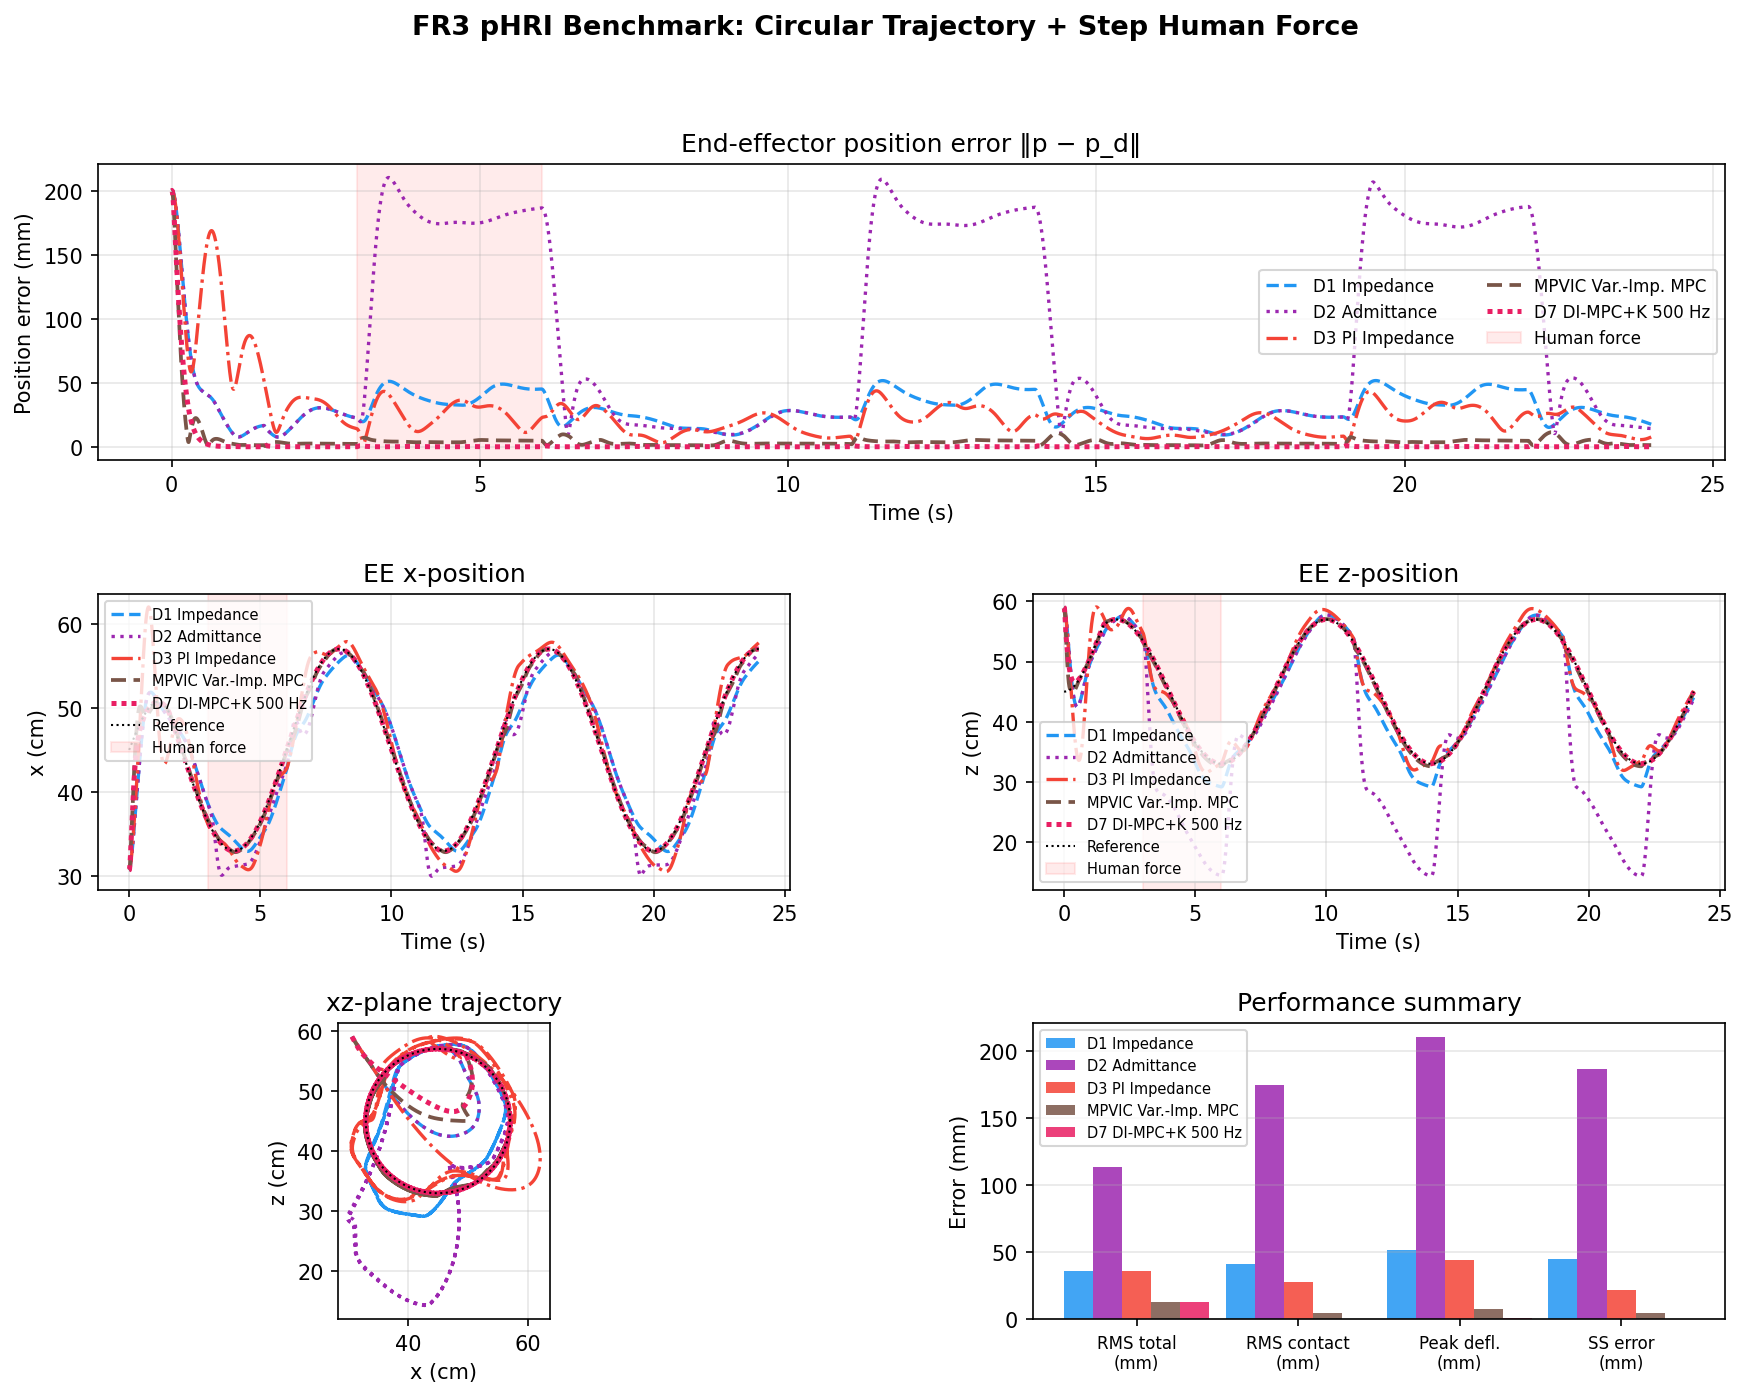
\includegraphics[width=0.8\columnwidth]{figures/mpc_comparison_results.png}
  \caption{Benchmark I --- Circular trajectory under 15\,N step pHRI.
           For visibility the plot shows D1/D2/D3/D7 (corresponding to
           C1/C2/C3/C7) plus the predictive variable-impedance MPVIC
           baseline; Table~\ref{tab:bm1} reports the full ablation. The
           final D7 controller achieves near-zero steady-state error and
           sub-millimeter peak deflection, while MPVIC---though predictive---retains
           a visible steady-state offset.}
  \label{fig:bm1}
\end{figure}

The comparison isolates five mechanisms:

\begin{itemize}[leftmargin=*,itemsep=1pt,topsep=2pt]
\item \textbf{Kalman augmentation removes steady-state error (C4 vs.\
C5).} With QP rate and horizon held fixed, folding $\hat d$ into the
free response drives steady-state error below 0.05\,mm --- down from
2.8\,mm over C4 and 44.8\,mm over C1; only the disturbance estimate
differs between C4 and C5, isolating offset-free cancellation directly.
\item \textbf{A large early gain, but gain-confounded (C1 vs.\ C4).}
With no disturbance model at all, C4's QP still cuts contact-window RMS
from 41.1 to 2.2\,mm ($19\times$) and peak deflection from 51.8 to
2.9\,mm. C1's nominal $K_d=300$\,N/m is a design choice, not C4's
realized closed-loop gain (Remark~\ref{rem:gains}), so this comparison
does not separate predictive look-ahead from a stiffer realized gain; a
matched-gain, horizon-length ablation is left to future work.
\item \textbf{Adapting stiffness alone is not enough (MPVIC vs.\ C5).}
MPVIC uses the \emph{same} $\hat d$ as C5 but only to schedule
stiffness, cutting contact RMS to 4.5\,mm --- better than every
reactive baseline --- yet it retains a 4.8\,mm steady-state error,
since a finite apparent stiffness can only bound deflection at
$e_\infty=-K^{\star-1}\hat d\neq0$. Offset-free cancellation
(Theorem~\ref{thm:zss}) removes this residual entirely ($\sim$140$\times$).
MPVIC is our own discrete-stiffness scheduler in the family of
\cite{liu2025model,roveda2019optimal}, not a reproduction of a specific
published algorithm; its stiffness set and force penalty have not been
swept for sensitivity.
\item \textbf{Rate and estimation are largely orthogonal (C4--C7).}
Raising the QP rate from 100 to 500\,Hz mainly shrinks the
zero-order-hold transient; adding the Kalman estimator mainly removes
the steady-state error. C7 combines both and gives the lowest
contact-window RMS, peak deflection, and steady-state error of any
controller; its total RMS (12.6\,mm, averaged over the whole cycle) is
marginally higher than C4/C5's (11.4\,mm), since the faster rate
sharpens the contact transient without improving free-motion tracking.
\item \textbf{Admittance yields by design (C2).} Its 174.7\,mm
contact-window RMS is close to the equilibrium prediction
$15/100=150$\,mm, the expected behavior of intentional compliance.
\end{itemize}

\textbf{Empirical joint-limit avoidance by the dual soft barrier
(boundary test).}
A 20\,cm radius circle pushes the arm toward its workspace boundary
(Table~\ref{tab:safety}, Fig.~\ref{fig:safety}), exercising the soft
null-space barrier and workspace projection only; the final CBF filter
(Theorem~\ref{thm:invariance}) is not engaged or logged here.

\begin{itemize}[leftmargin=*,itemsep=1pt,topsep=2pt]
\item Classical impedance violates the 5\% margin; the dual-barrier MPC
avoids it, holding a 0.083--0.084 margin at both 100 and 30\,Hz ---
joint-limit avoidance is insensitive to QP rate.
\item The elevated MPC RMSE (12.4\,mm vs.\ 0.3\,mm at $R=12$\,cm)
reflects the workspace projection deliberately trading tracking
accuracy for clearance near the boundary.
\end{itemize}

\begin{table}[!t]
\caption{Boundary Test, $R=20$\,cm Circle}
\label{tab:safety}
\renewcommand{\arraystretch}{1.0}
\centering
\footnotesize
\setlength{\tabcolsep}{2.5pt}
\footnotesize
\begin{tabular}{@{}lccc@{}}
\toprule
\textbf{Controller} & \textbf{RMSE [mm]} & \textbf{Min margin} & \textbf{Result}\\
\midrule
IMP         & 26.97 & 0.049 & \textsf{LIMIT VIOLATION}\\
MPC (C5, 100\,Hz QP) & 12.35 & 0.084 & \textsf{AVOIDED}\\
MPC (C5, 30\,Hz QP)  & 11.21 & 0.083 & \textsf{AVOIDED}\\
\bottomrule
\end{tabular}
\end{table}

\begin{figure}[!t]
  \centering
  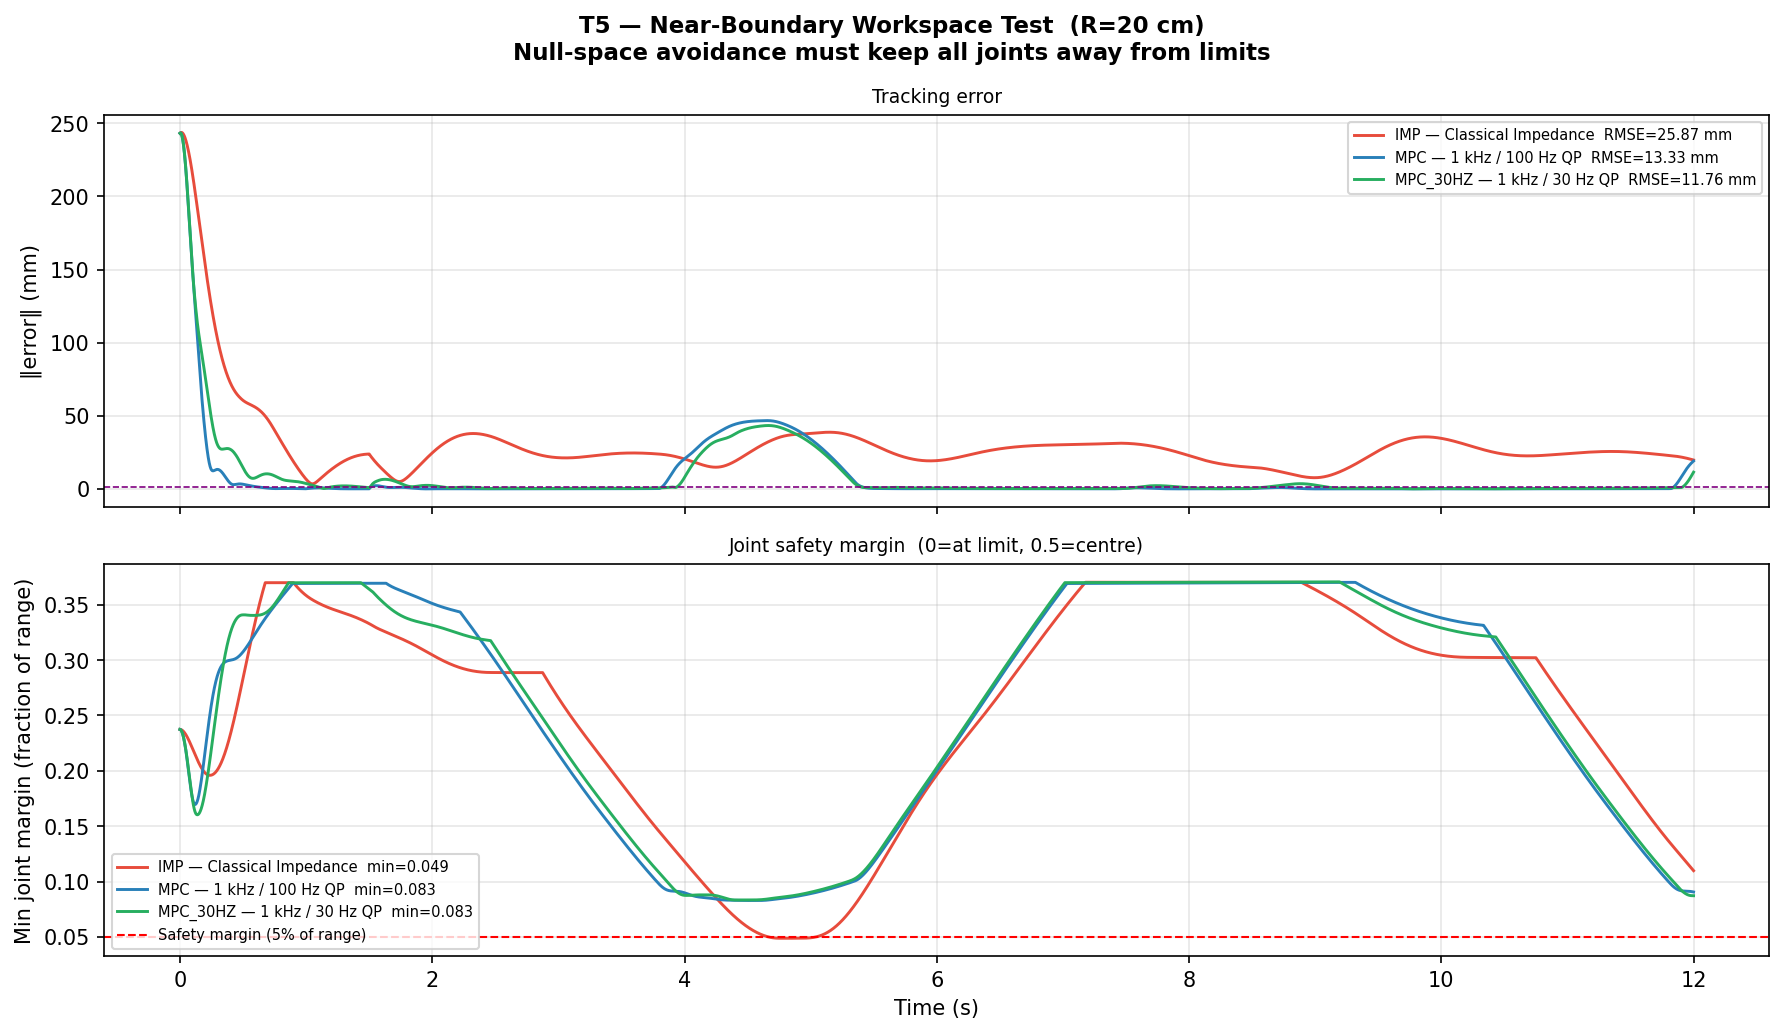
\includegraphics[width=0.8\columnwidth]{figures/trajectory_boundary.png}
  \caption{Boundary test ($R=20$\,cm).
           Classical impedance violates the 5\% joint margin;
           the dual-barrier MPC maintains a fractional joint margin
           $\geq0.084$ throughout.
           Elevated RMSE (12.4\,mm) reflects the workspace projection
           intentionally offsetting $p_d$ by up to 6\,cm to maintain
           joint-limit clearance.}
  \label{fig:safety}
\end{figure}

\textbf{Robustness to position-measurement noise and model mismatch.}
The architecture depends on a Kalman estimator, sensitive to
measurement noise, and on Layer-1 cancellation, sensitive to model
error, so we stress-test each independently: the plant is always the
true model, and only the controller's inputs (added EE-position noise)
or its model (the feedforward inertia $\Lambda$, scaled up by 0 to
30\% relative to the true plant) are perturbed. Velocity noise, sensing
latency, and force-sensor noise are not modeled here.

\begin{table}[!t]
\caption{Robustness of MPC+Kalman (100\,Hz QP)}
\label{tab:robust}
\renewcommand{\arraystretch}{1.0}
\centering
\footnotesize
\begin{tabular}{cccc}
\toprule
\multicolumn{4}{l}{\emph{(a) EE position noise --- 10\,N step, SS error
(5 seeds)}}\\
\midrule
noise $1\sigma$ & 0\,mm & 1\,mm & 2\,mm / 5\,mm\\
SS err (mm) & 0.08 & $0.19\pm.03$ & $0.36\pm.04$ / $0.89\pm.07$\\
\midrule
\multicolumn{4}{l}{\emph{(b) Inertia mismatch --- free-circle RMSE (mm)}}\\
\midrule
inertia error & 0\% & +10\% / +20\% & +30\%\\
Kalman on  & 0.24 & 0.24 / 0.23 & 0.23\\
Kalman off & 0.96 & 0.87 / 0.80 & 0.74\\
\bottomrule
\end{tabular}
\end{table}

\begin{itemize}[leftmargin=*,itemsep=1pt,topsep=2pt]
\item Under a 10\,N step disturbance (top table; steady-state error as
mean $|e|$ over the last 0.5\,s of the push, mean $\pm$ std over 5
measurement-noise seeds), even an unrealistically large 5\,mm
($1\sigma$) position noise leaves steady-state error below 1\,mm, with
the transient peak rising only modestly (1.6 to 2.2\,mm) --- the
integrating Kalman state averages out zero-mean sensor noise.
\item Under free-space XZ-circle tracking with a deliberately wrong
feedforward inertia (bottom table), Kalman-augmented RMSE stays
essentially invariant to up to 30\% inertia error ($0.24\to0.23$\,mm),
since the resulting feedforward force error is slowly varying and is
absorbed by $\dhat$ --- the empirical counterpart of the exactness
remark (Section~III). Disabling the Kalman exposes the mismatch
(0.74--0.96\,mm, 3--4$\times$ worse), confirming that it is the
disturbance state, not the nominal model, that confers the robustness.
\end{itemize}

\textbf{Further experiments and parameters.} The supplementary material
reports three further ablations run under the same codebase: a
time-varying-force horizon-prediction study (Table~S4), a human-force
magnitude and shape sweep (Table~S5), and an impedance-backbone
ablation, \textbf{C8}, that degrades gracefully rather than collapsing to
bare feedforward when the QP's corrective authority is curtailed
(Table~S6) --- along with the full numeric parameter table (Table~S1).

% ----------------------------------------------------------
\section{Discussion and Conclusion}

This paper argued that safe pHRI is best designed by predicting
\emph{interaction dynamics} directly (Definition~\ref{def:id}):
operational-space feedforward cancellation exposes a linear
interaction-dynamics backbone --- a double-integrator reduction of the
interaction error --- with configuration dependence confined to
$B_d(\rho_k)$, turning compliance, tracking, disturbance rejection, and
safety into properties of one 30-variable convex QP. Within its scope
the controller recovers classical impedance in the unconstrained,
disturbance-free limit (Theorem~\ref{thm:equiv}), is offset-free under
constant bounded force (Theorem~\ref{thm:zss}), and is quadratically
stabilizable by one fixed feedback gain over a certified polytope of
configurations (Theorem~\ref{thm:workspace}). On a Franka FR3 in MuJoCo
it reduces steady-state error under a sustained 15\,N force by
$>$800$\times$ over classical impedance, cuts free-space circle RMSE by
$77$--$97\times$, keeps joints inside their limits at the workspace
boundary, and is robust to position-measurement noise and up to $30\%$
inertial mismatch; the supplementary material adds a second waypoint-hold
benchmark, a disturbance-rate sweep, and an impedance-backbone ablation
(Sec.~S8) that degrades gracefully rather than collapsing when the
optimizer's corrective authority is curtailed.

The framework is one realization, not a universal replacement for
admittance-style co-manipulation. Because the interface needs only
$M$, $C\dot q+G$, and $J_v$,
it ports across torque-controlled arms by substituting the robot model
and joint-limit parameters; and because it reduces contact to an
analytic linear model with a fixed transition matrix, it may serve as a
dynamics prior for model-based physical AI, letting a learned model
capture only the residual uncertainty of intent, contact, and
environment. The next validation step is real FR3 pHRI testing with
synchronized tracking, force-estimation, CBF-residual, and energy-tank
logs.

% ----------------------------------------------------------
\bibliographystyle{IEEEtran}
\bibliography{references}

\end{document}
